\subsection{Exercício 8}
Relativamente ao exercício 8, era pedido que se estudasse a capacidade preditiva relativamente ao atributo Ativo usando os métodos: 
\begin{itemize}
\item Árvore de Decisão
\item Rede Neuronal
\item K-vizinhos-mais-próximos
\end{itemize} 

Relativamente à árvore de decisão, para a criação do modelo, utilizou-se a técnica \textbf{hold out} para criação de amostras de treino e de teste. As amostras foram criadas a partir do data frame Clientes DataSet com proporções de 70\% para treino e 30\% para teste. Após isso utilizou-se a função \textbf{rpart} para se fazer a árvore utilizando o atributo "Ativo" com a sintaxe "Ativo ~ ." uma vez que o ponto final representa todos os atributos. De seguida fez-se o plot desta mesma árvore como se observa na Fig. 8. Por fim, fez-se a previsão com a árvore e os dados de teste. 

\begin{figure}[htbp]
\centerline{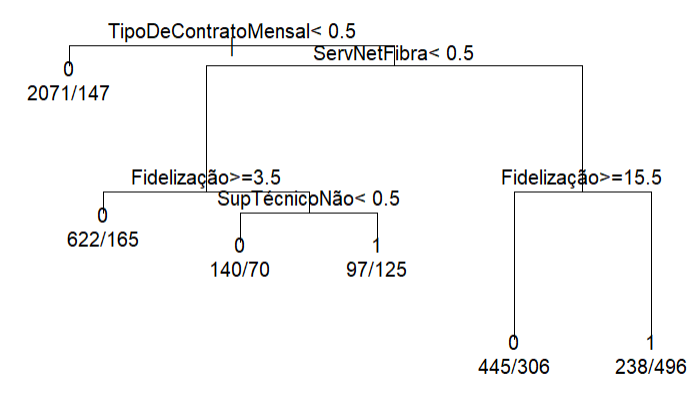
\includegraphics[width=9.5cm]{images/ex8_arvore_de_decisao.png}}
\caption{Árvore de decisão relativamente ao atributo Ativo.}
\label{ex8_arvore_de_decisao}
\end{figure}

Relativamente à rede neuronal, utilizamos a técnica \textbf{hold out} para criação de amostras de treino e de teste através dos dados normalizados da mesma forma que na alínea acima descrita. Esta rede neuronal foi testada com números nós diferentes, estando atualmente a ser utilizado com c(12, 6, 3). Testou-se apenas com 1 nó e verificou-se que a accuracy era bastante menor por isso optou-se pelo número de nós referido anteriormente. De seguida utilizou-se a função \textbf{neuralnet} com o atributo "Ativo" com a sintaxe "Ativo ~ ." e fez-se o sumário dos resultados ao invocar a "result\_matrix". Por fim, criou-se um data.frame com os dados de teste excluindo o atributo a ser estudado ("Ativo") e fez-se a previsão utilizando a função \textbf{compute}. Ainda assim, para se avaliar o modelo desnormalizaram-se os dados e calculou-se a raiz quadrada do erro médio (RMSE) obtendo o resultado \textbf{0.5027684}.

Por fim, e quanto aos K-vizinhos-mais-próximos, realizou-se o \textbf{hold out} e criaram-se matrizes de exemplos de teste e treino juntamente com um vetor com as respostas de cada observação do conjunto de treino. Após isso realizou-se a previsão do atributo "Ativo" utilizando-se o \textbf{KNN para a regressão} que retorna o valor médio dos k vizinhos mais próximos. No final retirou-se o k mínimo e máximo que deram \textbf{45} e \textbf{47} respetivamente e observaram-se os seguintes plots nas Fig. 9 e 10.

\begin{figure}[htbp]
\centerline{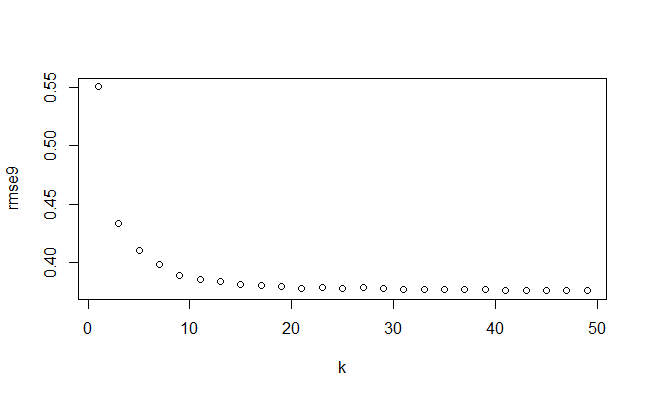
\includegraphics[width=9.5cm]{images/ex8_c_plot_min.png}}
\caption{Plot do atributo Ativo através do método K-vizinhos-mais-próximos para o valor mínimo}
\label{ex8_c_plot_min}
\end{figure}

\begin{figure}[htbp]
\centerline{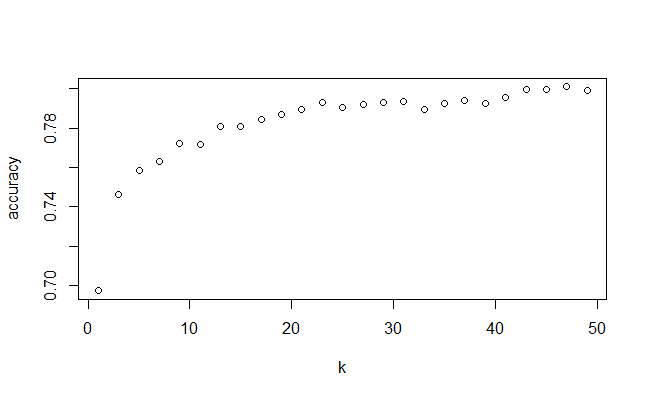
\includegraphics[width=9.5cm]{images/ex8_c_plot_max.png}}
\caption{Plot do atributo Ativo através do método K-vizinhos-mais-próximos para o valor máximo}
\label{ex8_c_plot_max}
\end{figure}